\chapter{Datacenter network model} \label{model}

In this chapter I describe common models of networks and data-centers as well as describe the model I implemented.

\section{Datacenter background} \label{model-dc}

\subsection{Network configuration} \label{model-network}

% A lot of this section is a mess
Most \datacenters \rotornet\cite{handley_re-architecting_2017}\opera \manya{the convention is to combine multiple citations into one}
There are anywhere from 5 to 50 servers in a rack, each connected to a switch typically at the top, giving it the common name "Top of Rack switch" or ToR. \manya{this sentence seems broken at the beginning: most datacetenrs There are}
A "small" \datacenter may have around 5,000 machines, large ones up to 250,000 or more. \manya{please add citation for all of these numbers}% TODO citation?

The racks themselves are connected together through different fabrics, and switch technologies.
The topology and technologies behind these is extremely varied \cite{kassing_beyond_2017}, and the subject of extensive research \opera\rotornet (TODO Xpander). \manya{please address all TODO cites. please cite more papers since the sentence says "extensive research"} % TODO cite

CLOS networks, or fat-trees, are a common topology in data-centers \manya{stay consistent: datacenter vs. data center vs. data-center} today \cite{singh_jupiter_2015}\cite{noauthor_reinventing_2019}\cite{noauthor_introducing_2014}.
They consist of a hierarchy of switches, with their bandwidth equally split up and down the hierarchy.
For cost-reduction purposes, it is common to have the first layer, from the servers to the ToR switch to be oversubscribed: the servers are able to send more traffic than the rack can handle. \manya{citation is needed}

\begin{figure}[h]
    \centering
    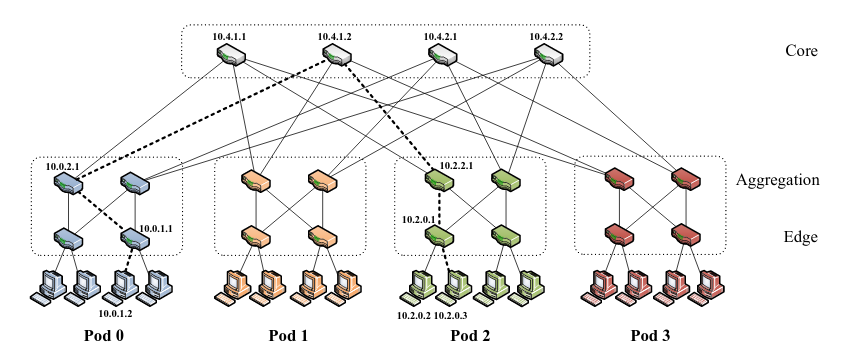
\includegraphics[width=\textwidth]{fat-tree}
    \label{fig:fat-tree}
    \caption{An example of a fat-tree topology from \cite{al-fares_scalable_2008}}
\end{figure}

The typical bandwidth vary but are in the 10Gbps to 100Gbps scale for server to ToR and ToR to ToR links \manya{which links?}.
Some networks assume different link speeds between the ToRs than from server to ToR \manya{cite}, others are uniform \manya{cite}.

The propagation delays, or `time to first byte', involved are often extremely small, on the order of tens of nanoseconds. \manya{cite. i don't think this claim is correct. RTTs are in the order of microseconds (store and fw on the switches takes time). look at latest sigcomm papers to find a citation.}\olivia{fixed latency -> propagation delay}


\subsection{Traffic modelling} \label{model-traffic}

There are a few well studied \datacenter traffic models (datamining \manya{cite}, websearch \manya{cite}, Chen Stefan Manya paper \manya{???? please remove sentences like this}, more), with a common takeaway being that \datacenter traffic is hard to predict.

Traffic distribution can be broken down into multiple dimensions: overall load, skeweness, and flow size distribution.


Overall load corresponds to how much traffic is being offered onto the network relative to how much capacity the network has.
It is important to note that this does not mean that the network is able to serve 100\% load, most networks are overwhelmed far before.
For example, if it takes 4 hops for a packet to get to a destination, traffic is essentially being sent 4 times, making it possible for loads above 25\% to saturate the network. \manya{this is not entirely true. it depends on timing and how they collide. please tone it down. we don't want someone reading this thesis to cite your thesis to say you claim \datacenters cannot handle load above 25\% out of context} \olivia{should be toned down now}

The traffic may be fairly uniform, each sender and receiver being involved in traffic all around the \datacenter, or very concentrated, with a few "hot" racks being very active with each other, the rest of the \datacenter quiet. \manya{again, this depends on timing granularity that you are observing the traffic. please clarify.} \olivia{added extra sentence}
These patterns can also be very different based on the timing granularity that they are being measured on. %cite
Describing these patterns can become quite complex, as there may be multiple "hot" regions mostly not interacting with each other.
Throughout this thesis,
%and in most of the literature
\manya{cite}\olivia{removed "most of lit" claim}
we are concerned about uniform traffic. \manya{please cite this claim or tone it down. we don't want someone to cite your thesis and say you claimed most of the \datacenter research focuses on uniform traffic. have you read most \datacenter papers to verify this is true? if so, cite them one by one to substantiate your claim. if not, don't make a claim we can't back up.}
\olivia{removed wild claim}

Finally, the flow size distribution corresponds to how big each flow is expected to be \cite{alizadeh_data_2010} \manya{the sentence should be complete without the citation.}.
Some workloads, such as websearch, consists mostly of many small flows.
Others, such as datamining, are comparatively much bigger.
Machine working loads also typically create a large demand, for example in a ring, using all the networking resources available.

\section{Simulation Model} \label{model-sim}

The \datacenter model used by Rustasim was chosen to emulate closely that of Opera \opera \manya{cite}, to allow for comparison and verification of the results.

The model used in Rustasim \ref{rustasim}, consists of two actor types: routers and servers, and three model-level event types: \code{packet}, \code{flow} and \code{timeout} events.
The servers are organized in racks, themselves interconnected through a user-chosen topology.

A \code{packet} event carries with it the corresponding packet and signals the arrival of that packet to the actor who then forwards it along appropriately.
If the packet carried by the event arrives at its destination, it is acked. 
If the packet is an ack arriving back at the sender, the flow reacts appropriately.\\

\code{Flow} events are received directly by servers and indicate the start of a new flow at that server.
\code{Timeouts} are received by the senders themselves and may cause a packet to be retransmitted if it hasn't been acknowledged.

Following with Opera's design \manya{?}\olivia{removed unecessary detail} the link speeds are all 10Gbps.
The latencies in the Opera simulator are set to 0 from server to ToR, and 500ns from ToR to ToR.
Unfortunately, conservative scheduling algorithms are unable to make progress with 0 latency, so I've set all latencies to be 500ns.
This has a measurable impact on the completion time of very small flows, where latency is the main contributor, but otherwise does not impact the results.
This is discussed more in section \ref{replication}.


\subsection{TCP} \label{model-tcp}

In this model, due to limited time, I implemented an extremely limited version of TCP with a fixed congestion window of size 30 \manya{this is a very unrealistic TCP. tone down your claim and say due to lack of time I only implemented ...}.
%similar to choices Opera makes \manya{please tone this down. we know opera has NDP as its congestion control so they might not like our characterization that opera mostly uses cwnd 30}. 
Although it is possible to implement a more realistic version of TCP, this simple version replicated the results of the Opera simulator on the specific runs we were interested in.
Congestion control can have a large effect on network performance, and even if this limited congestion control process works here, it should not be relied upon for further research.
\manya{tone this down. we didn't run an extensive set of evaluations. congestion control is extremely important and it's too dangerous to claim a cwnd = 30 is good enough}
\olivia{toned down, added warning}
